\subsection{棱锥}\label{subsec:2-2}

\begin{enhancedline}

\subsubsection{棱锥的概念和性质}

帆布帐篷、金字塔(图 \ref{fig:ltjh-2-11})等物体,都给我们以棱锥的形象。

\begin{figure}[htbp]
    \centering
    \begin{minipage}[b]{10cm}
        \centering
        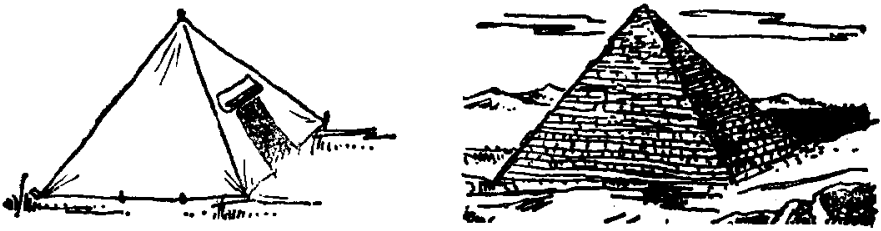
\includegraphics[width=10cm]{../pic/ltjh-ch2-11.png}
        \caption{}\label{fig:ltjh-2-11}
    \end{minipage}
    \qquad
    \begin{minipage}[b]{4cm}
        \centering
        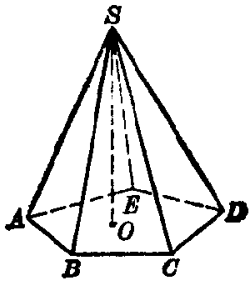
\includegraphics[width=3cm]{../pic/ltjh-ch2-12.png}
        \caption{}\label{fig:ltjh-2-12}
    \end{minipage}
\end{figure}

有一个面是多边形,其余各面是有一个公共顶点的三角形,由这些面所围成的几何体叫做\zhongdian{棱锥}(图 \ref{fig:ltjh-2-12}),
这个多边形叫做\zhongdian{棱锥的底面},其余各面叫做\zhongdian{棱锥的侧面}。
相邻侧面的公共边叫做\zhongdian{棱锥的侧棱},各侧面的公共顶点叫做\zhongdian{棱锥的顶点},
顶点到底面的距离叫做\zhongdian{棱锥的高}。 如图 \ref{fig:ltjh-2-12} 中的棱锥,多边形 $ABCDE$ 是底面,
三角形 $SAB$、$SBC$ 等是侧面,$SA$、$SB$ 等是侧棱,$S$是顶点,$SO$ 是高。

\begin{figure}[htbp]
    \centering
    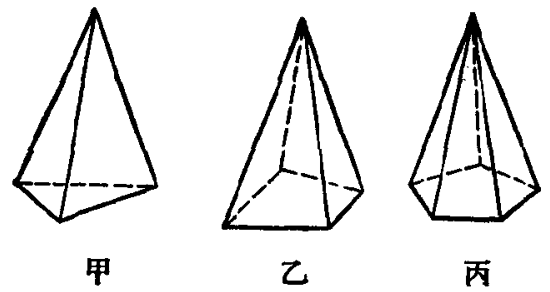
\includegraphics[width=10cm]{../pic/ltjh-ch2-13.png}
    \caption{}\label{fig:ltjh-2-13}
\end{figure}

棱锥用表示顶点和底面各顶点,或者底面一条对角线端点的字母来表示。
例如,棱锥 $S{-}ABCDE$,或者棱锥 $S{-}AC$。

棱锥的底面可以是三角形、四边形、五边形、…,因此我们把这样的棱锥分别叫做三棱锥(图 \ref{fig:ltjh-2-13} 甲)、
四棱锥(图 \ref{fig:ltjh-2-13} 乙)、五棱锥(图 \ref{fig:ltjh-2-13} 丙)、…。

如果一个棱锥的底面是正多边形,并且顶点在底面的射影是底面中心,这样的棱锥叫做\zhongdian{正棱锥}。

正棱锥有下面一些性质:

(1)\zhongdian{各侧棱相等,各侧面都是全等的等腰三角形。}各等腰三角形底边上的高相等,它叫做\zhongdian{正棱锥的斜高};

(2)\zhongdian{棱锥的高、斜高和斜高在底面上的射影组成一个直角三角形;
棱锥的高、侧棱和侧棱在底面上的射影也组成一个直角三角形}(图 \ref{fig:ltjh-2-14})。

\begin{figure}[htbp]
    \centering
    \begin{minipage}[b]{7cm}
        \centering
        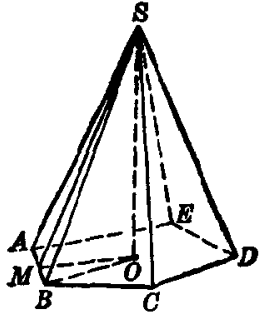
\includegraphics[width=4cm]{../pic/ltjh-ch2-14.png}
        \caption{}\label{fig:ltjh-2-14}
    \end{minipage}
    \qquad
    \begin{minipage}[b]{7cm}
        \centering
        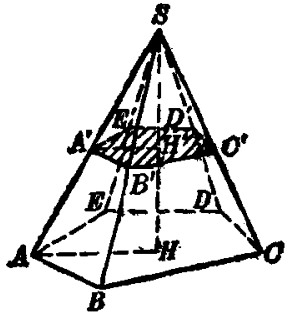
\includegraphics[width=4.5cm]{../pic/ltjh-ch2-15.png}
        \caption{}\label{fig:ltjh-2-15}
    \end{minipage}
\end{figure}

关于一般棱锥,有下面一个重要性质:

\begin{dingli}[定理][dl:lz-jm-mjb]
    如果棱锥被平行于底面的平面所截,那么截面和底面相似,并且它们面积的比等于截得的棱锥的高和已知棱锥的高的平方比。
\end{dingli}


已知:如图 \ref{fig:ltjh-2-15},在棱锥 $S{-}AC$ 中,$SH$ 是高,截面 $A'B'C'D'E'$ 平行于底面,并与 $SH$ 交于 $H'$。

求证:$\text{截面}\; A'B'C'D'E' \xiangsi \text{底面}\; ABCDE$,
并且 $\dfrac{S_{A'B'C'D'E'}}{S_{ABCDE}} = \dfrac{SH'\,^2}{SH^2}$。

\zhengming 因为截面平行于底面,所以 $A'B' \pingxing AB$, $B'C' \pingxing BC$, $C'D' \pingxing CD$, …。
因而 $\angle A'B'C' = \angle ABC$, $\angle B'C'D' = \angle BCD$, …。
又因为过 $SA$、$SH$ 的平面与截面和底面分别交于 $A'H'$ 和 $AH$,

$\therefore$ \quad $A'H' \pingxing AH$,得

\hspace{5em} $\dfrac{A'B'}{AB} = \dfrac{SA'}{SA} = \dfrac{SH'}{SH}$。

同理 \hspace{3em} $\dfrac{B'C'}{BC} = \dfrac{SH'}{SH}$,…。

$\therefore$ \quad $\dfrac{A'B'}{AB} = \dfrac{B'C'}{BC} = \cdots = \dfrac{SH'}{SH}$。

因此,$\text{截面}\; A'B'C'D'E' \xiangsi \text{底面}\; ABCDE$。

$\therefore$ \quad $\dfrac{S_{A'B'C'D'E'}}{S_{ABCDE}} = \dfrac{A'B'\,^2}{AB^2} = \dfrac{SH'\,^2}{SH^2}$,



\begin{wrapfigure}[8]{r}{4.5cm}
    \centering
    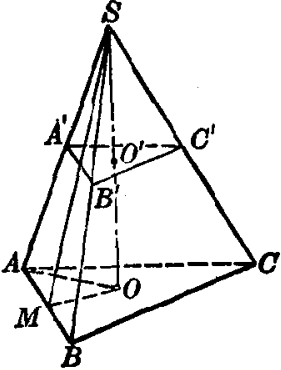
\includegraphics[width=4cm]{../pic/ltjh-ch2-16.png}
    \caption{}\label{fig:ltjh-2-16}
\end{wrapfigure}

\liti 如图 \ref{fig:ltjh-2-16},已知正三棱锥 $S{-}ABC$ 的高 $SO = h$,斜高 $SM = l$。
求经过 $SO$ 的中点平行于底面的截面\footnote{象这样过高的中点平行于底面的截面叫做中截面。}
$\triangle A'B'C'$ 的面积。

\jie 连结 $OM$、$OA$. 在 $Rt \triangle SOM$ 中, $OM = \sqrt{l^2 - h^2}$。

因为棱锥 $S{-}ABC$ 是正棱锥,所以点 $O$ 是正三角形 $ABC$ 的中心。

$AB = 2 AM = 2 \cdot OM \cdot \tan 60^\circ = 2\sqrt{3} \cdot \sqrt{l^2 - h^2}$,

$S_{\triangle ABC} = \dfrac{\sqrt{3}}{4} AB^2 = \dfrac{\sqrt{3}}{4} \times 4 \times 3 (l^2 - h^2) = 3\sqrt{3} (l^2 - h^2)$。

根据一般棱锥截面的性质,有
$$ \dfrac{S_{\triangle A'B'C'}}{S_{\triangle ABC}} = \dfrac{h'\,^2}{h^2} = \exdfrac{1}{4} \juhao $$

$\therefore$ \quad $S_{\triangle A'B'C'} = \dfrac{3\sqrt{3}}{4} (l^2 - h^2)$。


\begin{lianxi}

\xiaoti{底面是正多边形的棱锥是正棱锥吗?}

\xiaoti{求证:正棱锥各侧面与底面所成的二面角都相等。}

\end{lianxi}



\subsubsection{正棱锥的直观图的画法}

正棱锥的直观图由底面和顶点所决定。正棱锥底面的画法与直棱柱的底面画法相同,
顶点和底面中心的距离,等于它的高。下面以正五棱锥为例,说明正棱锥的直观图的画法。


\liti 画一个底面边长为 5 cm,高为 11.5 cm 的正五棱锥的直观图。比例尺是 $\exdfrac{1}{5}$。

\huafa (1)画轴 \quad 画 $x'$ 轴、$y'$轴、$z'$轴,使 $\angle x'O'y' = 45^\circ$,
$\angle x'O'z' = 90^\circ$(图 \ref{fig:ltjh-2-17} 甲)。

(2)画底面 \quad 按 $x'$轴、$y'$ 轴画正五边形的直观图 $ABCDE$,按比例尺,
取边长等于 $5 \div 5 = 1 \;(\limi)$,并使正五边形的中心对应于点 $O'$。

(3)画高线 \quad 在 $z'$ 轴上,取 $O'S = 11.5 \div 5 = 2.3$ (cm)。

(4)成图 \quad 连结 $SA$、$SB$、$SC$、$SD$、$SE$,并加以整理,
就得到所要画的正五棱锥的直观图(图 \ref{fig:ltjh-2-17} 乙)。

\begin{figure}[htbp]
    \centering
    \begin{minipage}[b]{8cm}
        \centering
        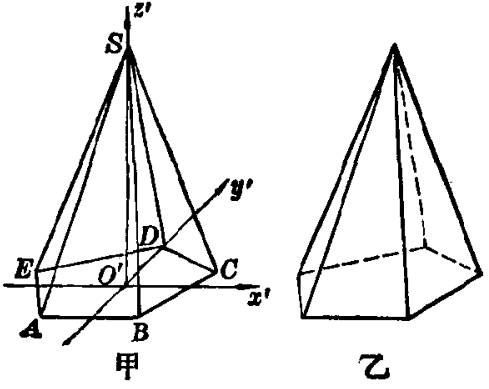
\includegraphics[width=8cm]{../pic/ltjh-ch2-17.png}
        \caption{}\label{fig:ltjh-2-17}
    \end{minipage}
    \qquad
    \begin{minipage}[b]{7cm}
        \centering
        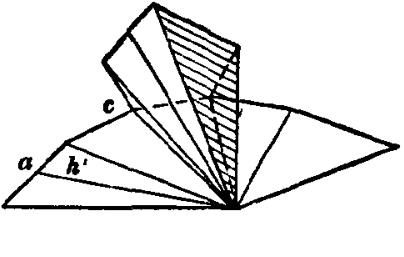
\includegraphics[width=7cm]{../pic/ltjh-ch2-18.png}
        \caption{}\label{fig:ltjh-2-18}
    \end{minipage}
\end{figure}

\subsubsection{正棱锥的侧面积}

棱锥的侧面展开图是由各个侧面组成的,展开图的面积就是棱锥的侧面积。
设正棱锥的底面边长为 $a$,周长为 $c$,斜高为 $h'$,则展开图(图 \ref{fig:ltjh-2-18})
的面积等于 $n \cdot \exdfrac{1}{2} ah' = \exdfrac{1}{2} ch'$。
由此得到下面的定理:

\begin{dingli}[定理][dl:zlj-cmj]
    如果正棱锥的底面周长是 $\bm{c}$,斜高是 $\bm{h'}$,那么它的侧面积是
    \begin{center}
        \framebox[10em]{$\bm{S_\text{正棱锥侧} = \exdfrac{1}{2} ch'}$。}
    \end{center}
\end{dingli}

棱锥的全面积等于侧面积与底面积的和。

\begin{wrapfigure}[5]{r}{5cm}
    \centering
    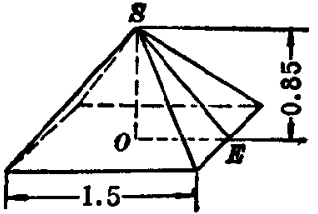
\includegraphics[width=5cm]{../pic/ltjh-ch2-19.png}
    \caption{}\label{fig:ltjh-2-19}
\end{wrapfigure}

\liti 设计一个正四棱锥形冷水塔塔顶,高是 0.85 m,底的边长是 1.5 m,
制造这种塔顶需要多少平方米铁板(保留两位有效数字)?

\jie 如图 \ref{fig:ltjh-2-19}, $S$ 表示塔顶的顶点,$O$ 表示底的中心,则 $SO$是高。 设 $SE$ 是斜高。

在直角三角形 $SOE$ 中,根据勾股定理得

$SE = \sqrt{\left(\dfrac{1.5}{2}\right)^2 + 0.85^2} \approx 1.13 \; (\mi)$。

$\therefore$ \quad $S_\text{正棱锥侧} = \exdfrac{1}{2} ch' = \exdfrac{1}{2} (1.5 \times 4) \times 1.13 \approx 3.4\;(\pfm)$。

答:制造这种塔顶需要铁板约 $3.4\;\pfm$。


\begin{lianxi}

\xiaoti{已知正六棱锥的底面边长为 6 cm,高为 15 cm,画它的直观图,比例尺为 $\exdfrac{1}{3}$。}

\xiaoti{一个正三棱锥的侧面都是直角三角形,底面边长是 $a$。求它的全面积。}

\end{lianxi}

\end{enhancedline}
